\chapter{Results \& Evaluation} \label{Evaluation}

This chapter covers the evaluation of the developed payloads and defence mechanisms. 


\section{Payloads}

It is difficult to find an objective, quantitative measure of the effectiveness of a payload. It is influenced by too many outside factors and the specific context it is deployed in. However, it is possible to qualitatively evaluate whether or not it can reach its own specific goal, discounting any factors of the bigger picture of the attack, such as whether the information was useful or the success of planting the hardware. This section will discuss whether the payloads introduced in chapter \ref{Methodology} achieve their declared goal. Within this aspect, there can be a distinction between reliability and speed. Both of these factors are heavily influenced by the circumstances surrounding the attacked host. Speed specifically may have to be adjusted to the computational power of the target and reliability depends heavily on how well this speed is chosen. Too little wait jeopardizes the entire attack, and long delays may produce overhead. However, the more time overhead the more reliable the payload in different situations, since it will work on more and older computers. Reliability can also be impacted by the other processes running on the computer, such as Bad USB-specific defences, antivirus software, Updates etc. . To be able to make some claims as to the flexibility (and thereby reliability) of these attacks, this evaluation will be carried out on multiple devices, specifically including computers in which the payloads have never been executed before. The following computers were used;

\begin{itemize}
    \item Microsoft Surface Laptop 4, Processor: 11th Gen Intel(R) Core(TM) i7-1185G7 @3.00GHz, 16.0 GB installed RAM running Windows 11 Home version 23H2 (Used for payload development), without any additional Antivirus or Bad USB protection
    \item MSI Stealth 16 Studio A13V, Processor: 13th Gen Intel(R) Core(TM) i7-13700H @2.40 GHz, 32 GB installed RAM running Windows11 Home version 23H2, without any additional antivirus or BAD USB protection.
    \item family home computer
    \item silvan?
\end{itemize}
    
In the following, this section will go through all the payloads and describe their execution on the above-mentioned devices. For every evaluation, the computers were unlocked, connected to the internet, and Bluetooth turned off. All running applications and background processes, including Teams, Outlook, Vanguard, Spotify, etc., were closed unless otherwise mentioned. Every target device's keyboard layout was set to Swiss ISO. The payloads were manually executed through a separate device. 

\subsubsection{Register Email Forwarding}

GOAL: Enable Email forwarding to a desired Email address as an attempt to gather intelligence and eavesdrop on conversations. \\
PREREQUISITES: The new Outlook version has to be installed on the target and the desired email must be logged in. Furthermore, the email for forwarding has to be configured in the payload. 

Already on the first execution of this payload on the MSI laptop a common problem appears; Outlook requires an update to operate. 

\begin{figure}[H]
    \centering
    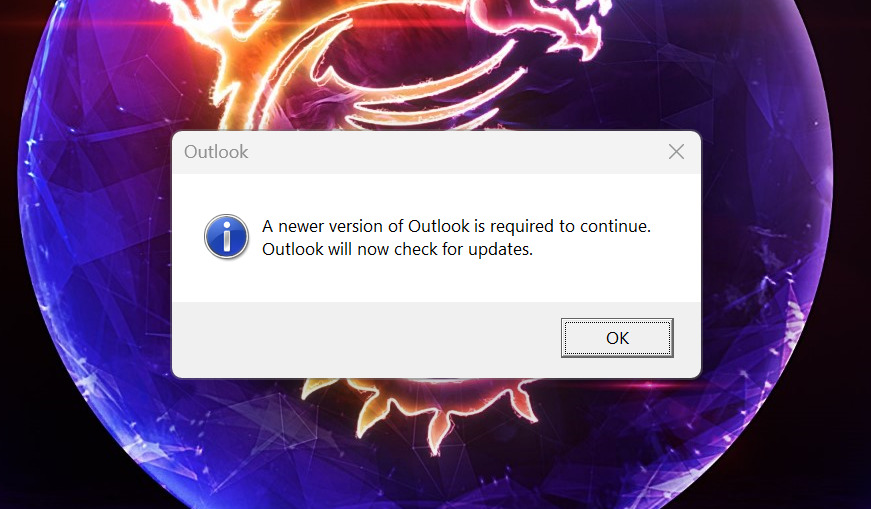
\includegraphics[width=0.5\linewidth]{visuals/outlook_requires_update.jpeg}
    \caption{Error Message after executing Forwarding Payload on MSI laptop}
    \label{fig:builtInTeensy}
    \cite{farhiMalboardNovelUser2019}
\end{figure}


Another big challenge with this payload is its UI focus. It requires a lot of settings menu navigation which is very time-sensitive. Short delays are detrimental here. Even for the MSI laptop which has the most compute of the tested devices, an especially long delay for opening Outlook and a delay of around 300ms between every navigation step is necessary to ensure that every TAB and ARROW input is correctly placed. \\
On the Microsoft Surface laptop, the attack worked as expected, which can be attributed to the fact that it was built while continuously being tested on this device. For none of the other test objects did the payload work out of the box, each would require updates, new logins or even lack the new Outlook completely. 

The conclusion for this payload is that it is not versatile and indeed requires a rather specific set of circumstances to work. Its UI focus makes this even harder since delays have to be high to accommodate the long loading times of an application like Outlook. If it works correctly, however, the payload can be very powerful and useful for gathering intelligence. 


\subsubsection{Disable Windows Event Logging}

GOAL: Disable Windows Event logging to hide possible traces another attack might leave. \\
PREREQUISITES: Windows 11

This payload has two versions; UI and CLI-based approaches, as discussed in chapter \ref{Implementation}. For the UI-based version, the usual problems occur; loading times, pop-up problems, and unforeseen reactions by the host. However, since this time the payload navigates through Windows Settings panels and not Outlook, some more continuity and speed can be expected. There are no server calls to be made that influence loading times, instead the process should be more straightforward. 
The Command Line Version should be even more reliable. It contains fewer steps and therefore less margin for error. It is expected to run smoothly on all test subjects.

The first execution of the UI-based approach proved once again its flakiness; Disabling Widows event logging on the MSI laptop would have also stopped another process, which caused the pop-up to confirm the action. This was not foreseen by the payload and therefore interrupted the process to the point where it exited the settings panel by selecting 'cancel' instead of 'apply' thereby ruining its progress. A second execution successfully stopped Windows event logging, since the pop-up did not appear again. However, it failed to close the settings window, leaving a trail of the attack. The navigation on the other side, was more reliable than what could be observed with the email forwarding payload which is as expected. \\
What was unexpected were language setting problems. When testing the payload on the TODO gaming desktop, it ran into problems because the search did not yield Windows event logging, but instead 'Windows Defender Advanced'. The payload would have to be adjusted to find the German 'Windows-Ereignisprotokoll'. After this adjustment, however, the next problem occurred; since the User did not have administrator rights, the settings options were greyed out and the payload had no chance of succeeding. \\
The payload worked well on the Surface Laptop, as expected since it was developed on it.

The CLI approach yielded much better results succeeding on the first try on the MSI laptop. As well as working on the custom-built gaming computer after adjusting the payload to enter the administrator password. As expected it also worked well on the Microsoft Surface Laptop. This result solidifies the superiority of a command line approach as opposed to navigating user interfaces. 


Conclusively it can be said that this payload works very well when applying the CLI approach. The UI version can work as well but requires a lot of fine-tuning, administrator access, and English as the system language. 



\subsubsection{Extract SSH hashes}

GOAL:\\ Extract SSH hashes from default storage on a device and send them to a command and control (C\&C) server.
PREREQUISITES: Windows 11 and a running C\&C server, in this case, Dropbox. Administrator rights are required

Since this script is working with default Windows settings, there are not a lot of challenges to be expected. On the MSI laptop, it worked flawlessly after some adjustments on the delays for opening the terminal. Since administrator access is not given on the custom gaming computer, the payload had to be adjusted to include the administrator password. With this adjustment, it was able to run successfully. The best results were again on the Windows Surface Laptop, where it executed flawlessly. 


\subsubsection{Extract Private Key Files}

GOAL: Find files that have extensions commonly used for private key files and send them to a C\&C server. \\
PREREQUISITES: Knowledge about the file system

This payload needs an entry point, some path to a local folder from which it can search through the files. If this is chosen too generally there may be permission issues. The entry point also heavily influences the time this payload takes to execute since it determines how many files the loop has to go through. The longer the script takes to execute, the easier it is to spot. \\
Since this payload does not require admin privileges one challenging step of opening an admin terminal is eliminated. One unexpected factor for errors is the validity length of the Dropbox access token. It expires within 4 hours. This means that in between saving the payload to the cable and the execution not more than those few hours may elapse. It was not a problem to adjust the payload for manual testing, however, this eliminates a C\&C server like Dropbox for boot scripts with unknown execution times. \\

The payload generally worked well on the Microsoft Surface laptop; its file system is known and an adequate entry point could be chosen. The execution was a success on the MSI laptop and the custom desktop as well. These good results could be due to the fact that apart from starting PowerShell, there are no loading times that can throw off the execution of the payload. Even waiting for the loop to end was not a problem; although delays were not adjusted to the expected search time, PowerShell still recognized and executed the command after finishing the loop.



\subsubsection{Steal Web Session Cookies}

GOAL: Figure out the target's default browser, then steal the web session cookies. \\
PREREQUISITES: None

This payload is pretty straightforward. Nevertheless, challenges for its flexibility arise. Executing the payload on the Microsoft Surface device went expectedly well, however, upon execution on the MSI laptop an error message occurred. Although the default browser on both of these devices is set to Firefox, their versions differ. While the Surface laptop had a slightly older version ( 129.0.1) the MSI laptop ran on the newest release, 129.0.2. This is reflected in the path to their cookies file. The .2 version stores the cookies at '\\Mozilla\\Firefox\\Profiles\\dpsymep9.default-release\\cookies.sqlite'  while .1 stores them at 'Mozilla\\Firefox\\Profiles\\umva4gfp.default-release\\cookies.sqlite' . This unexpected little, but crucial detail, derailed the execution of the script on the MSI laptop. The Chrome cookies path seems to be more robust; it worked without adjustments after changing the default for the MSI laptop to Chrome. The same problem occurred with the execution on the custom-built computer; it is running Firefox version wkbzpjnx. A more flexible version of this payload would check for versions and insert them as variables in the string, similar to how it does it with the Username environment variable. 

Apart from the version issues this payload performed well and as expected. 


\subsubsection{Iteratively End Processes}



GOAL: Certain processes should be ended as soon as they are detected as running. In whitelist mode, all programs except a few should be ended when they are detected as running.\\
PREREQUISITES: Windows 11, no admin rights required


This payload worked surprisingly well on the very first try. The MSI laptop posed no problem at all, not even delay adjustments had to be made. It worked as expected, terminating processes from the whitelist. As expected, the payload executed well on the Microsoft Surface, and on the desktop as well. \\
The only aspect that posed some problems was the minimizing of the window after the execution of the payload. It seemed that the 'ALT SPACE' keypresses were not registered by the device and were not acted upon. On every device, the window was simply left open creating an obvious drawback for this payload; it is easy to spot and stop manually. 

\subsubsection{Schedule Processes}

GOAL: Schedule a job on the target device to execute a chosen script at a chosen time. \\
PREREQUISITES: Windows, administrator privileges

In order to test this payload, I set the script of the job to be \verb|Get-Process|. Execution on the MSI laptop worked well. However, it is important to note, that executing the payload twice back to back will generate an error because the process 'ProcessJob' is already registered. To confirm the registration of the job, the Windows Scheduler Application can be used. The process should be listed under task scheduler library -> Microsoft -> Windows -> PowerShell -> ScheduledJobs. \\
Execution on the Surface Laptop went without issues as well. A challenge for the desktop is that the payload requires admin privileges. After adjusting the payload to enter the admin password, the payload is executed without any issues. 

\begin{figure}[H]
    \centering
    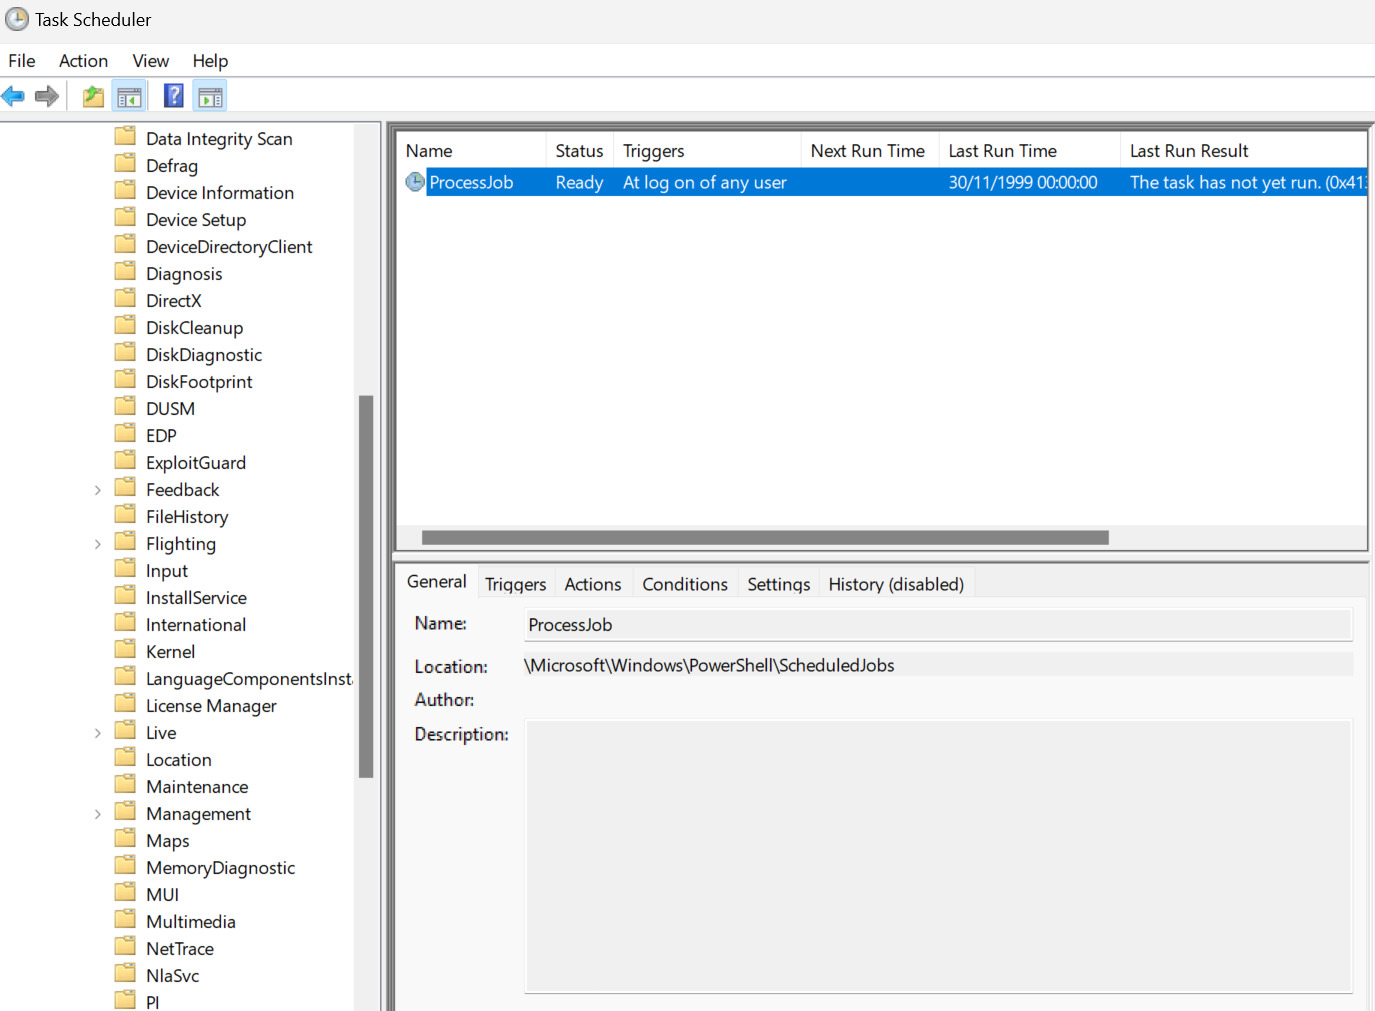
\includegraphics[width=0.5\linewidth]{visuals/task_scheduler_MSI.jpeg}
    \caption{Task Scheduler on the MSI laptop after successful registration of the Job}
    \label{fig:TaskScheduler}
\end{figure}



\subsection{Conclusion Attack Evaluation}


\section{Defence Evaluation} \label{defence evaluation}


This section will evaluate the performance of the defence script. To illustrate the progress a payload makes before it is interrupted, this thesis proposes a new metric. It measures the success of the payload in executed keystrokes divided by the total keystrokes in the payload. Executed keystrokes include commands such as \verb|ENTER| or \verb|LEFTARROW|and commands such as \verb|GUI R| are counted as two keystrokes. Variable length inputs, such as the email address to forward to in ''Register Email Forwarding`` are not considered in the total keystrokes of a payload. The benefit of this metric is that it represents how close the payload got to executing completely, thereby achieving the attacker's goal. Its biggest disadvantage is that it does not reflect the actual success of the payload, since it does not take into account whether the input happened at the correct place and time. For example, a payload could execute 100\% of its keystrokes, but if there was an error along the way the payload likely still failed. This is why the metric is complemented by a qualitative description of the result to describe the end state of the payload. In the case of 100\% execution with an error along the way, it would state that the PowerShell script experienced an error and did not execute successfully. 

 A spam payload is introduced to get a baseline for the performance of the executions without any delays or unknown factors. It's a simple script that does nothing besides set the keyboard language and input a large number of ''a``s. Listing \ref{lst:a_spam} shows an excerpt of this script. 


\begin{lstlisting}[caption={Excerpt: write 2670 'a's without delays},label=lst:a_spam, captionpos=b]
DUCKY_LANG DE_CH
STRING aaaaaaaaaaaaaaaaaaaaaaaaaaaaaaaaaaaaaaa
\end{lstlisting}

The execution of this script against all the following versions of the defence script provides a comparative value for the other payloads.

The two components of the defence script are evaluated separately: first, this chapter looks at the enumeration pattern detection, and then it deals with the two options for the rate limiter.


\subsection{Enumeration Pattern Detection}

This subsection will describe a series of experiments to evaluate the speed of the enumeration pattern analysis (EPA). For these experiments, every payload is run against the defence script with the rate limiter disabled, as shown in Listing \ref{lst:start_script_dr}.

\begin{lstlisting}[caption={start Defense Script with Rate Limiter disabled},label={lst:start_script_dr}, captionpos=b]
 py .\omg_detection.py "USBDeview file path" -dr
\end{lstlisting}

This defence is not expected to have any differences in performance between the payloads; it acts solely on the information from the cable itself, and what happens after the enumeration is not of any concern. \\
The following list explains the qualitative and quantitative progress every payload made.

\begin{itemize}
    \item  \emph{''a`` spam}: 23 ''a``s were written by the payload before it stopped. | 23/2670
    \item  \emph{Register Email Forwarding:} The interruption happened after the Windows Search Menu was opened and 'outlook(new) typed in.  |  14/70 
    \item  \emph{Disable Windows Event Logging CLI:}  Execution stopped at the pop-up to confirm user privileges. | 3/88
    \item  \emph{Disable Windows Event Logging UI:} The attack reached the Windows run window and entered ''services.msc`` | 14/47
    \item  \emph{Extract Hashes:}  The payload progressed until the pop-up window confirming user privileges. | 3/728 
    \item  \emph{Extract Private Key Files:}  | Although no input was made, the payload did manage to open PowerShell. 14/1024
    \item  \emph{Steal Websession Cookies:} The attack was stopped right after opening PowerShell. | 16/1157
    \item  \emph{Iteratively End Processes:} Again the cable was disconnected after opening PowerShell. | 16/386
    \item  \emph{Schedule Processes:} The disconnect happened during the User Account Control popup to confirm admin rights. | 3/209
\end{itemize}

\begin{table}[h]
\centering
\begin{tabular}{|c|c|}
\hline
Name & EPA  \\
\hline
''a`` spam & 23/2670 \\
\hline
Register Email Forwarding & 14/70 \\
\hline
Disable Windows Event Logging CLI & 3/88 \\
\hline
Disable Windows Event Logging UI & 14/47 \\
\hline
Extract Hashes & 3/728  \\
\hline
Extract Private Key Files & 14/1024 \\
\hline
Steal Websession Cookies & 16/1157 \\
\hline
Iteratively End Processes & 16/386 \\
\hline
Schedule Processes & 3/209 \\
\hline
\end{tabular}
\caption{Table of executions rates for EPA}
\label{table:EPA_results}
\end{table}

Every execution was interrupted successfully before it could make any impact, often before any of its intentions were clear. The effect of delays becomes obvious when comparing scripts that require admin rights with those that don't. That first group has many delays at the start of the script to open menus and wait for pop-ups. This gives the script a lot of time to react and disconnect the cable, hence the very low execution rates. The other group, on the other hand, uses the widows run menu to open PowerShell or Windows Services which is more input-heavy compared to the navigation of the first group. Start-heavy payloads are therefore able to input more keystrokes before the disconnect. In either case, the defence is a success, it detects the attack in 100\% of cases before anything can be executed. \\
However, still, the execution rates are not zero and are proof of the latency of the defence script. The result of the spam payload shows, that it is possible to enter 23 consecutive keystrokes into a target machine before this defence would step in. Fortunately for possible victims, this is only a theoretical scenario; every payload in practice would have to waste time with delays and could not get near the 23 keystrokes, as visible in the results chart of Listing \ref{table:EPA_results}\


\subsection{Rate Limiter}

This section will determine which values for the time window and interarrival time analysis respectively are best suited in defense against the newly formulated attacks.\\
As a baseline, the speed of input for O.MG cables is determined. Theoretically, the O.MG cables are advertised to have input speeds of 120 keys/sec for the basic version and 890 keys/sec for elite. The O.MG cable used for development in this thesis is an elite cable. The ''a``spam payload introduced in the introduction to Section \ref{defence evaluation} is used to test this. It consists of 2670 ''a``s that should be printed out without any delays into a notepad. Since the elite cable should be able to input 890 keystrokes per second the complete execution is expected to take 3 seconds. The elapsed time is measured using the Epoch Arrival time of the first UBR\_INTERRUPT frame carrying the correct HID data as captured by Wireshark and the last. \\
Running the payload three times results in a consistent measured execution time of 43.0 seconds. This is equivalent to 69.0 keystrokes/second, 12.9 times slower than expected. it is therefore much closer to what has been established as humanly possible in section \ref{Methodology} at 25 keystrokes/second. TODO; find out why \\
Typing time can be categorized into two components: the interval between keystrokes and the duration each key is pressed. The duration of each keypress can be determined using the timestamps from the input frames; subtracting the timestamp of the initial press signal from the release frame timestamp provides the press duration. This data yields a key press duration time of 7.9 to 8.1 milliseconds. Taking the 43 seconds the O.MG cable took to input 2670 keystrokes and subtracting the press time for each of these keys: 43 - (0.008*2670) results in a total interarrival time of 21.64 seconds. Considering that over 2670 keystrokes there are 2669 interarrival slots, an interarrival time of 21.64/2669 = 0.0081 seconds, or 8.1 milliseconds for O.MG input can be derived. These calculations serve as the basis for establishing reasonable inputs for the rate limiter options in the following subsections.  

\subsubsection{Interarrival Time Analysis}


Interarrival Time Analysis (ITA) was implemented by \cite{neunerUSBlockBlockingUSBBased2018} who described a detection mechanism for what they call Rapid Keypress event sequence (RES). A RES would be detected every time a sequence \emph{s} of consecutive keypresses arrives with an interarrival time less than a defined threshold \emph{t} between each of them. They concluded that \emph{t} should be at 0.02 s with an \emph{s} of 3 to allow some averaging while ruling out false negatives for short attacks. To come to their conclusion, the paper assumes a minimum interarrival time for organically generated keypresses of 80ms, based on a study from 1985 \cite{umphressIdentityVerificationKeyboard1985}. It has to be kept in mind that this value might be outdated.

To test these assumptions the script can be run with the command shown in Listing \ref{lst:start_script_ita}


\begin{lstlisting}[caption={start Defense Script with ITA (0.02,3)},label={lst:start_script_ita}, captionpos=b]
 py .\omg_detection.py "USBDeview file path" -de --i "(0.02,3)
\end{lstlisting}

\begin{itemize}
    \item  \emph{Register Email Forwarding:} {''a`` spam}: 47 ''a``s were written by the payload before it stopped. | 47/2670
    \item  \emph{Register Email Forwarding:} The payload was interrupted after searching for Outlook(new) in the Windows Search Menu without opening it.  | 14/70 
    \item  \emph{Disable Windows Event Logging CLI:} Execution progressed until opening the power user menu to start PowerShell. | 2/88
    \item  \emph{Disable Windows Event Logging UI:} It reached the Windows Services settings, where it would navigate to disable the event logging. However, execution stopped before any navigation could take place.  | 14/47
    \item  \emph{Extract Hashes:} Opened PowerShell in administrator mode without making any input. | 5/728 
    \item  \emph{Extract Private Key Files:} The disconnect happened right after PowerShell was opened. | 16/1024
    \item  \emph{Steal Websession Cookies:} Identically to the private key file extraction, this payload ran until the PowerShell Window opened. | 16/1157
    \item  \emph{Iteratively End Processes:} This payload also reached PowerShell without being able to input anything. | 16/386
    \item  \emph{Schedule Processes:} Just like the previous three payloads, this payload was also able to open PowerShell and did not come further. | 5/209
\end{itemize}

In theory, this configuration (0.02 seconds averaged over 3 characters) should trigger a disconnect after the first 3 inputs; however, it takes until character 47 of the ''a`` spam payload to react, putting it at a 0.018\% execution rate. The reason for this is the latency of the defense script. Adjusting the configuration to average over 2 characters confirms this; the disconnect happens after 41 characters only 6 characters earlier. It is marginally faster because it can react one keystroke sooner, however the latency is so big that the effect of the adjustment is only small.

Delays in the payload unexpectedly improved the performance of the rate limiter; after the first keystrokes to open a menu or application, the pauses made sure that the program had time to react. Opening PowerShell as administrator starts with an input of 3 characters within 116 milliseconds, which results in an average interarrival time of 38 milliseconds, a value far above the threshold of 20 miliseconds  so then how tf is this even possible???
2 * 0.008 + 0.1

Since the average was over such a small number of characters, even opening the power user menu and selecting an option there (3 keys) already triggered the disconnect. Payloads that did not require administrator access, such as ``extract private key files'' made more progress, since they do not require navigating the confirmation pop up. However, this also relies on timing, with shorter delays, such as in ``Schedule Processes'' PowerShell could also be opened as administrator. 


\subsubsection{Time Window Analysis}

All payloads developed in the scope of this thesis start by opening a program such as PowerShell or some settings menu. Opening a PowerShell prompt without administrator permissions from the run window, takes a minimum of 12 keystrokes, opening via the poweruser menu only three. Opening an Admin window takes 5. 
An input of 3 keystrokes at 69 keystrokes/second takes 43.5 milliseconds, therefore the configuration to catch an input of 3 keystrokes would have to be 3 keystrokes in 0.0435 seconds.

A basic test simply writing only ''a``s without opening any programs or using any delays disconnects after inputting 64 characters. \\
It was not possible to trigger the rate limiter by spamming the keyboard manually.\\
In the following, this subsection describes how well this configuration works for detecting any of the newly developed payloads:

%py .\omg_detection.py "C:\Users\maaik\Downloads\usbdeview" -de --t "(0.0435,3)"

 \begin{itemize}
    \item  \emph{Register Email Forwarding:} Execution was disrupted after seraching for outlook(new) in the windows search menu. | 14/70
    \item  \emph{Disable Windows Event Logging CLI:} The payload was able to almost finish; running until the second to last line of the script, which would have disabled the logging. It was only 21 keystrokes short after having already typed 63 and waited for 3 seconds. | 63/88
    \item  \emph{Disable Windows Event Logging UI:}  It managed to open the Windows Service settings, identically to the ITA analysis. | 6/47
    \item  \emph{Extract Hashes:} The payload progressed 2 full lines into the PowerShell script. | 49/728
    \item  \emph{Extract Private Key Files:} This attack also executed until PowerShell without being able to make any input. | 16/1024
    \item  \emph{Steal Websession Cookies:} Identically to the ITA experiment, this payload progressed until PowerShell. | 16/1157
    \item  \emph{Iteratively End Processes:} This attack was also terminated right after opening PowerShell. | 16/386
    \item  \emph{Schedule Processes:} This payload stopped short only a few keystrokes from completion. It was interrupted 59 keystrokes before the point where ITA stopped the execution. | 68/209
\end{itemize}

Performance was mostly similar to ITA, however notably here ``Disable Windows Event Logging'' and ``Schedule Process'' nearly terminated and ``Extract Hashes'' was able to execute multiple lines of code. All of these payloads open the command line in administrator mode through the power user menu. 
The attacks that opened the command line through the run menu (``Steal Websession Cookies'', ``Extract Private Key Files'' , and ``Iteratively end Processe'')  were not able to write any commands to the PowerShell Window they opened. 

It is apparent that this configuration, while aiming to detect payloads that start with 3 to 5 keystrokes to open a terminal, does badly, specifically for those payloads while performing better for payloads with longer inputs at the start (i.e. opening a terminal with Windwos Run and \verb|powershell(.exe)|. This is most likely due to the delays; The concise way to open a administrator terminal through the power user menu requires delays; waiting for the menu to open, waiting for the confirmation window to pop up, waiting for the navigation to be registered. This way the rate limiter is not triggered, only when the longer inputs into the command line start does it jump into action. Since there is some delay in the defense script between the triggering input and the disconnect command, the payload manages to execute multiple lines.  A more concise attach might even execute fully before the cable is disconnected. 

As seen in listing \ref{open_powershell_admin} there are delays after every command, specifically delays that are longer than the considered time window. Therefore, every time a keystroke is recorded and triggers a time window check, there will be only one or two keystrokes in the 43 millisecond time window, the third keystroke will only be reached when the command line input actually starts. This begs the question, whether a maximum contingent of two keystrokes would be able to interrupt the payloads sooner by already detecting the very first input \verb|GUI X|. 

\begin{lstlisting}[caption={First 10 lines of ``Schedule Job'' Payload},label=lst:open_powershell_admin, captionpos=b]
    DUCKY_LANG DE_CH
    DELAY 50
    GUI x
    DELAY 100
    STRINGLN a
    DELAY 600
    LEFTARROW
    DELAY 50
    ENTER
    DELAY 2000
\end{lstlisting}

Therefore, the next experiment will explore how fast the payloads are detected when looking for inputs of 2 keystrokes. The Time Window for this analysis comes out to 28.98 milliseconds considering the 69 k/s input speed.\\
These are the results:

The ''a`` spam payload was interrupted after 41 characters, which is 23 characters and 35\% faster than before. A human spam test that included furiously hitting as many keys as fast as possible did not manage to trigger the rate limiter.

 \begin{itemize}
    \item  \emph{Register Email Forwarding:} Opened Windows Search and typed outlook(new) without opening it. | 14/70
    \item  \emph{Disable Windows Event Logging CLI:} The payload was stopped at the first 'e' of the second PowerShell script line. 36/88
    \item  \emph{Disable Windows Event Logging UI:} Progressed until Services Menu without navigating further. | 6/47
    \item  \emph{Extract Hashes:} The first c on the third line of the PowerShell script was the last letter before the execution of this attack was stopped. | 5/728
    \item  \emph{Extract Private Key Files:}  The attack progressed up to opening PowerShell without writing anything. | 16/1024
    \item  \emph{Steal Websession Cookies:} Identically to before, this payload managed to open PowerShell but did not advance further. | 16/1024
    \item  \emph{Iteratively End Processes:} This attack also succeeded in opening PowerShell. | 16/1024
    \item  \emph{Schedule Processes:} Progress was interrupted at character 25 of line two of the Powershell script. | 64/209
\end{itemize}

%py .\omg_detection.py "C:\Users\maaik\Downloads\usbdeview" -de --t "(0.0289,2)"

\subsection{Conclusion Defense Evaluation}

TODO draw conclusion from this once oyu have the metrics calculated


\begin{table}[h]
\centering
\begin{tabular}{|c|c|c|c|c|}
\hline
Name & EPA &  ITA(0.02,3) & TWA (0.0435, 3) & TWA (0.0289,2) \\
\hline
''a`` spam & 23/2670 & 47/2670 & 64/2670 & 41/2670 \\
\hline
Register Email Forwarding & 14/70 & 14/70 & 14/70 & 14/70 \\
\hline
Disable Windows Event Logging CLI & 3/88 & 2/88 & 63/88 & 36/88 \\
\hline
Disable Windows Event Logging UI & 14/47 & 14/47 & 6/47 & 6/47 \\
\hline
Extract Hashes & 3/728 & 5/728 & 49/728 & 5/728 \\
\hline
Extract Private Key Files & 14/1024 & 16/1024 & 16/1024 & 16/1024 \\
\hline
Steal Websession Cookies & 16/1157 & 16/1157 & 16/1157 & 16/1024 \\
\hline
Iteratively End Processes & 16/386 & 16/386 & 16/386 & 16/1024 \\
\hline
Schedule Processes & 3/209 & 5/209 & 68/209 & 64/209 \\
\hline
\end{tabular}
\caption{Table of executions rates for EPA, TWA and ITA}
\end{table}

Time Window Analysis can therefore be circumvented by adding many small delays between the commands or making them concise enough to be able to execute within the latency of the program. \\








